\documentclass[a4paper, 12pt]{article}

\usepackage{graphicx}
\usepackage{xcolor}
\usepackage{mdframed}
\usepackage { amsmath , amssymb , amsthm }
\usepackage[T2A]{fontenc}
\usepackage[utf8]{inputenc}
\usepackage[english,russian]{babel}

\graphicspath{{img/}}
\DeclareGraphicsExtensions{.pdf,.png,.jpg}


\title{Инженерная графика}
\author{Щербинин В.В}
\date{\today}

\begin{document}
\sffamily
\maketitle

\section*{Введение}

ЕСКД -- единая система конструкторской документации (устанавливает взаимосвязь правил по оформлению, конструированию, обращинию конструкторской документации)\\
"+":\\
1. Возможность взаимообмена конструкторской документации между предприятиями.\\
2. Стабилизация комплектности, исключающая дубрированость документов.\\
3. Возможность обеспечивать унификации при конструировании, разработке, проэктированиии комерческих изделий\\
4. Упращенная форма конструкторской документации.\\
5. Механизм и автоматизм обработки технической документации.\\
\newpage
\section{Методы проекции}

\subsection{Центральная проекция}
Для получения центральных проекций необходимо задаться плоскостью проекций H и центром проекций S.\\
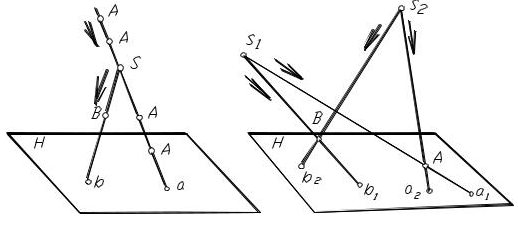
\includegraphics{eng1}\\
Центр проекций действует как точечный источник света, испуская проецирующие лучи. Точки пересечения проецирующих лучей с плоскостью проекций H называются проекциями. Проекций не получается, когда центр проецирования лежит в данной плоскости или проецирующие лучи параллельны плоскости проекций.\\

Свойства центрального проецирования:\\
1.Каждая точка пространства проецируется на данную плоскость проекций в единственную проекцию.\\
2.В то же время каждая точка на плоскости проекций может быть проекцией множества точек, если они находятся на одном проецирующем луче\\
3.Прямая, не проходящая через центр проецирования, проецируется прямой (проецирующая прямая – точкой).\\
4.Плоская (двумерная) фигура, не принадлежащая проецирующей плоскости, проецируется двумерной фигурой (фигуры, принадлежащие проецирующей плоскости, проецируются вместе с ней в виде прямой).\\
5.Трехмерная фигура отображается двумерной.\\
Глаз, фотоаппарат являются примерами этой системы изображения. Одна центральная проекция точки не дает возможность судить о положении самой Точки в пространстве, и поэтому в техническом черчении это проецированиепочти не применяется. Для определения положения точки при данном способе необходимо иметь две ее центральные проекции, полученные из двух различных центров. Центральные проекции применяют для изображения предметов в перспективе. Изображения в центральных проекциях наглядны, но для технического черчения неудобны.

\subsection{Параллельная проекция и их свойства}
Параллельное проецирование – частный случай центрального проецирования, когда центр проецирования перемещен в несобственную точку, т.е. в бесконечность. При таком положении центра проекций все проецирующие прямые будут параллельны между собой. В связи с параллельностью проецирующих прямых рассматриваемый способ называется параллельным, а полученные с его помощью проекции – параллельными проекциями. Аппарат параллельного проецирования полностью определяется положением плоскости проецирования (H) и направлением проецирования.\\

Свойства параллельного проецирования:\\
1.При параллельном проецировании сохраняются все свойства центрального проецирования, а также возникают новые:\\
2.Для определения положения точки в пространстве необходимо иметь две ее параллельные проекции, полученные при двух различных направлениях проецирования.\\
3.Параллельные проекции взаимно параллельных прямых параллельны, а отношение длин отрезков таких прямых равно отношению длин их проекций.\\
4.Если длина отрезка прямой делится точкой в каком-либо отношении, то и длина проекции отрезка делится проекцией этой точки в том же отношении .\\
5.Плоская фигура, параллельная плоскости проекций , проецируется при параллельном проецировании на эту плоскость в такую же фигуру.\\

Параллельное проецирование, как и центральное, при одном центре проецирования, также не обеспечивает обратимости чертежа.\\
Применяя приемы параллельного проецирования точки и линии, можно строить параллельные проекции поверхности и тела.\\

\subsection{Прямоугольное (ортогональное)проецирование}

\textbf{Прямоугольное проецирование} -- это частный случай параллельного проец при котором проецирующие прямые перпендикулярны плоскости проекции и параллельны друг-другу.
\\
Ортогональные проекции двух взаимно перпендикулярных прямых, одна из которых параллельны плоскоти проекций а другая не перпендикулярна ей взаимно перпендикулярны.\\
Преймущества:\\
1. простота\\
2. при ортогональном проецировании, при ряди условий удается сохранить форму и размеры фигуры.\\

\subsection{Проецирование на две взаимно перпендикулярные плоскости проекции}
Обратимость чертежа может быть обеспечена проецированием на две плоскости проекции.\\
%вставить рисунок взаимно перпендикулярных плоскостей

Состоит из фронтальной и горезонтальной плоскастей проекций, а линия пересечения называется осью проекции и называбт x или v/h.\\

В некоторых случаях удобней использовать:\\
%вставить фронтальную и профильные проекции

состоит из фронтальной и профильной плоскотей проекций, ось пересечения называется v/w.\\

Горизонтальные проекции точки называют прямоугольную проекцию точки на горизонтальную плоскость проекции.\\

%вставить рисунок проецирования v/h
обозначения: $ a $ на h , $ a' $ на v для точки $ A $\\
плоскость Q перпендикулярна плоскостям проекции и пересекает ось проекции x\\
Для того чтобы востановить положение A необходимо востановить перпендикуляры к плоскостям проекций в $a \quad a'$, на пересечении перпендикуляров находится точка A\\
Две параллельные проекции точки на различные плоскости проекции вполне определяют ее положение в пространстве, а значит проецирование на две ортогональных плоскости проекции обеспечивает обратимость чертежа для точки.\\

Эпюры Моджа:\\
%рисунок
Отрезок a'a называетс линией связи\\

\subsection{Проецирование на три взаимно перпендикулярные плоскости проекции}

%рисунок трех плоскостей проекции

называется V,H,W. Точка O - пересечение трех проекций.\\

Принято разрезать ось y\\

!!!Помнить про чертову прямую -45 градусов\\
При параллельных прямых все их проекции параллельны!!!\\

\section{Глава. Проецирование отрезка прямой линии}
\subsection{Проецирование отрезка прямой линии и деление его в заданном отношении}

Отрезки $a_p \quad b_p$ ледат в некоторой плоскости Q, эта плоскость перпендикулярна плоскости P, прямая, по которой плоскость Q пересекает плоскость P содержит точки AB\\

tckb njxrf ghbyflkt;bn ytrjve jnyjityb. nj tt ghjtrwbb ghbyflkt;fn jlyjbvvtyysv ghjtrwbzv jnhtprf и делят их в одном и томже отношении.%красиво
\\

\subsection{Положение прямой линии в отношении плоскостей проекции. Особые случаи положения прямой}
1. прямая не параллельна ни одной из плоскостей проекции(прямая общего положения)\\
2. прямая параллельны одной из плоскостей проекции или ей принадлежит(прямая частного положения)\\
3. параллельна двум плоскостям проекции и перпендикулярна третей(прямая частного положения)\\

Соответственно называется фронтальной или профильной прямой(в зависимости какой параллельна плоскости).\\
Если прямая перпендикулярна одной из плоскостей проекции то она называется проецирующей для этой плоскости(горизонтально,фронтально,профильно проецирующией)\\
Проецирующая прямая проецируется на соответствующиую плоскость проекции в точку.\\

\subsection{Определение натуральной велечины прямой, общего положения и углов его наклона к плоскостям проекции}

\subsection{Взаимное положение прямой}

Пересекающиеся прямые -- если прямые пересекаются то их одноименные проекции персекаются между собой а проекции точек пересечения лежат на одной линии связи. В системе VH справедливо для всях прямых кроме профильных и обратное утверждение, если точки пересечения одноименных проекций прямых лежат на одной линии связи то прямые пересекаются.\\
\[
	\frac{b' m'}{a' m'} = \frac{b m}{a m}	
\]
\[
	\frac{c' m'}{a' m'} = \frac{cm}{am}	
\]

Параллельные прямые -- если прямые параллельны то их одноименные проекции параллельны между собой. Для прямых общего положения справедливо и обратное, если проекции прямых общего положения в системе двух плоскостей проекции параллельны то сами прямые также параллельны. Если одноименные проекции прямых параллельны одной из осей проекции то прямые параллельны при условии параллельности одноименных проекций на той плоскости проекций которой параллельны прямые.\\

Скрещивающиеся прямые не имеют общих точек. Проекции скрещивающихся прямых пересекаются но точки пересечения проекций не лежат на одной линии связи.\\

\section{Глава. Плоскость}
\subsection{Положение плоскости относительно плоскостей проекции}

Плоскость можно задать разными способами:\\
-3мя точками, нележащими на одной прямой\\
-прямой и точкой, взятой вне этой прямой\\
-двумя пересекающимися прямыми\\
-двумя параллельными прямымы\\
-какая-либо плоская фигура\\

Положение плоскости по отношению к плоскотям проекции:\\
1)Плоскость не перпендикулярны плоскостям проекций(плоскость общего положения)\\
2)плоскость может быть перпендикулярна одной плоскости проекции(плоскости часного положения, проецирующие плоскости)\\
3)плоскость может быть перпендикулярна двум плоскостям проекции(плоскости часного положения, проецирующие плоскости)\\

След плоскости -- это линия пересечения плоскости с плоскостью проекции.\\

Для плоскости перпендикулярной плоскости H горизонтальный след PH распологается под углом к оси проекции X соответсвующе углу наклона этой плоскости к фронтальной плоскости проекции, а фронтальный след перпендикулярно оси X. Для плоскости перпендикулярной плоскости V фронтальный след распологается под углом к оси x соотвествующим углу наклона этой плоскости к плоскости H а горизонтальный след перпендикулярен оси X. На чертежах след перпендикулярный оси проекции не изображают.\\

Любая геометрическая фигура, лежащая в проецирующей плоскости, проецируется на соотвествующую плоскость проекции в прямую линию.\\
Плоскость перпендикулярна двум плоскостям проекции и параллельны третей.\\

\subsection{Прямая и точка в плоскости}
задачи:\\
1) Проведения прямой в плоскости\\
2) Построение  точки в некоторой плоскости\\
3) ...\\
4) Проверка принадлежности точки плоскости\\

Если точка принадлежит плоскости то ее проекции лежат на проекции прямой принадлежащей плоскости.\\
















\end{document}